\documentclass{standalone}
\usepackage{tikz}
\usetikzlibrary{patterns, positioning}
\usepackage[sfdefault]{ClearSans} %% option 'sfdefault' activates Clear Sans as the default text font
\usepackage[T1]{fontenc}

\begin{document}
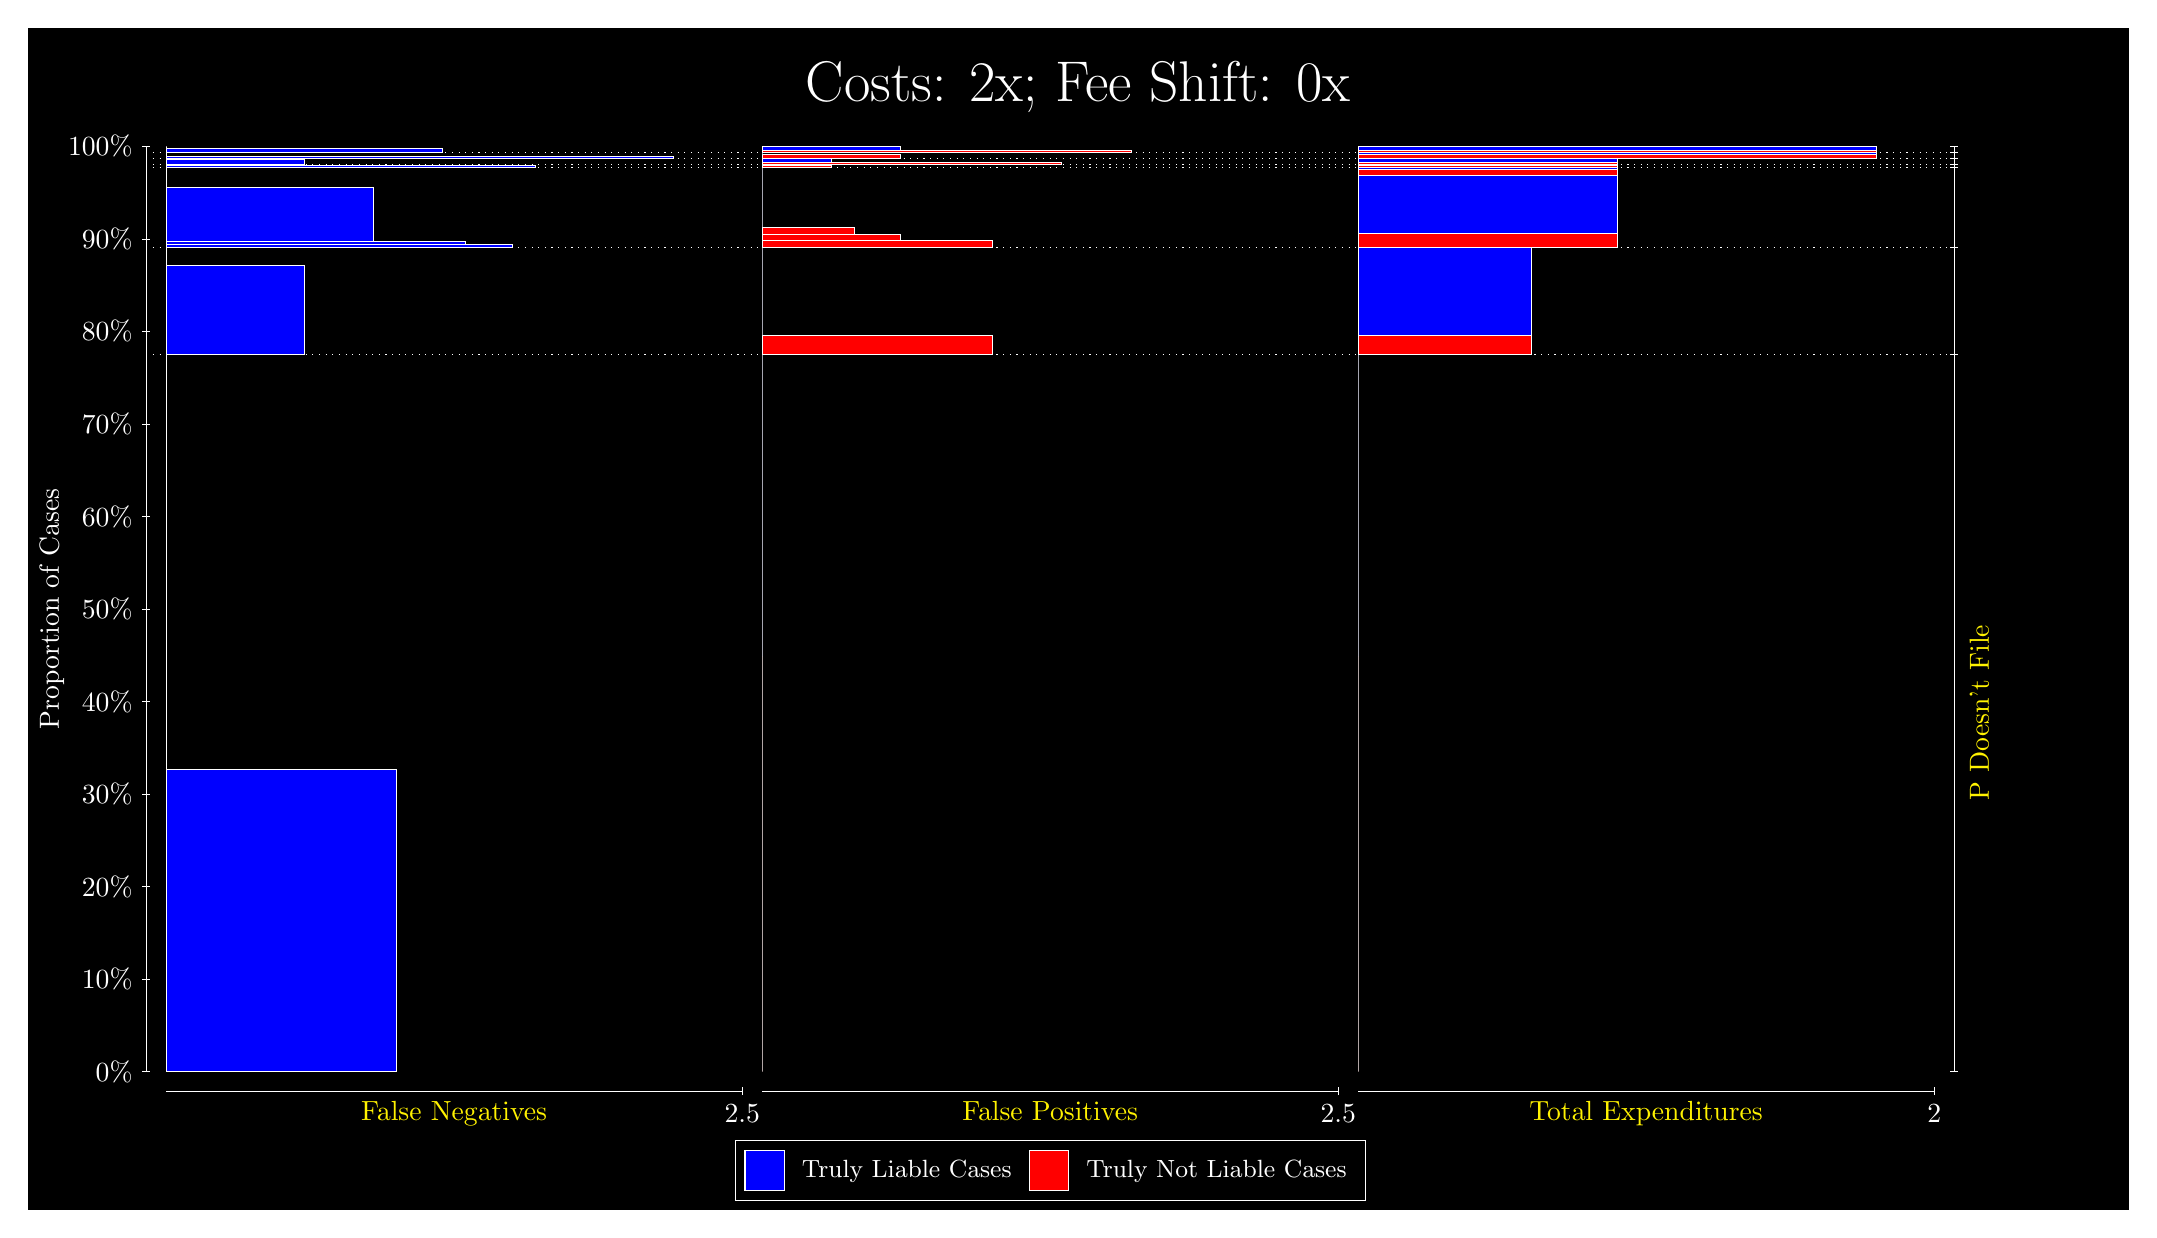
\begin{tikzpicture}
\draw[fill=black] (0,0) rectangle (26.667,15);
\draw[text=white] (0,13.5) rectangle (26.667,15) node[midway] {\huge Costs: 2x; Fee Shift: 0x};
\draw[white, very thin] (1.5,1.75) -- (1.5,13.5);
\node[rotate=90, text=white, anchor=center] at (0.3, 7.625) {Proportion of Cases};
\draw[white, very thin] (1.45,1.75) -- (1.55,1.75);
\node[text=white, anchor=east] at (1.45, 1.75) {0\%};
\draw[white, very thin] (1.45,2.925) -- (1.55,2.925);
\node[text=white, anchor=east] at (1.45, 2.925) {10\%};
\draw[white, very thin] (1.45,4.1) -- (1.55,4.1);
\node[text=white, anchor=east] at (1.45, 4.1) {20\%};
\draw[white, very thin] (1.45,5.275) -- (1.55,5.275);
\node[text=white, anchor=east] at (1.45, 5.275) {30\%};
\draw[white, very thin] (1.45,6.45) -- (1.55,6.45);
\node[text=white, anchor=east] at (1.45, 6.45) {40\%};
\draw[white, very thin] (1.45,7.625) -- (1.55,7.625);
\node[text=white, anchor=east] at (1.45, 7.625) {50\%};
\draw[white, very thin] (1.45,8.8) -- (1.55,8.8);
\node[text=white, anchor=east] at (1.45, 8.8) {60\%};
\draw[white, very thin] (1.45,9.975) -- (1.55,9.975);
\node[text=white, anchor=east] at (1.45, 9.975) {70\%};
\draw[white, very thin] (1.45,11.15) -- (1.55,11.15);
\node[text=white, anchor=east] at (1.45, 11.15) {80\%};
\draw[white, very thin] (1.45,12.325) -- (1.55,12.325);
\node[text=white, anchor=east] at (1.45, 12.325) {90\%};
\draw[white, very thin] (1.45,13.5) -- (1.55,13.5);
\node[text=white, anchor=east] at (1.45, 13.5) {100\%};

\draw[white, very thin] (24.457,1.75) -- (24.457,13.5);
\draw[white, very thin] (24.407,1.75) -- (24.507,1.75);
\node[anchor=west] at (24.407, 1.75) {};
\draw[white, very thin] (24.407,10.86) -- (24.507,10.86);
\node[anchor=west] at (24.407, 10.86) {};
\draw[white, very thin] (24.407,12.218) -- (24.507,12.218);
\node[anchor=west] at (24.407, 12.218) {};
\draw[white, very thin] (24.407,13.236) -- (24.507,13.236);
\node[anchor=west] at (24.407, 13.236) {};
\draw[white, very thin] (24.407,13.272) -- (24.507,13.272);
\node[anchor=west] at (24.407, 13.272) {};
\draw[white, very thin] (24.407,13.35) -- (24.507,13.35);
\node[anchor=west] at (24.407, 13.35) {};
\draw[white, very thin] (24.407,13.419) -- (24.507,13.419);
\node[anchor=west] at (24.407, 13.419) {};
\draw[white, very thin] (24.407,13.5) -- (24.507,13.5);
\node[anchor=west] at (24.407, 13.5) {};

\draw[white, very thin, fill=blue] (1.75,1.75) rectangle (4.6775,5.5828);
\draw[white, very thin, fill=red] (1.75,5.5828) rectangle (1.75,10.86);
\draw[white, very thin, fill=blue] (1.75,10.86) rectangle (3.5065,11.984);
\draw[white, very thin, fill=red] (1.75,11.984) rectangle (1.75,12.218);
\draw[white, very thin, fill=blue] (1.75,12.218) rectangle (6.1413,12.258);
\draw[white, very thin, fill=blue] (1.75,12.258) rectangle (5.5558,12.291);
\draw[white, very thin, fill=blue] (1.75,12.291) rectangle (4.3848,12.981);
\draw[white, very thin, fill=red] (1.75,12.981) rectangle (1.75,13.236);
\draw[white, very thin, fill=blue] (1.75,13.236) rectangle (6.4341,13.253);
\draw[white, very thin, fill=red] (1.75,13.253) rectangle (1.75,13.272);
\draw[white, very thin, fill=blue] (1.75,13.272) rectangle (3.5065,13.33);
\draw[white, very thin, fill=red] (1.75,13.33) rectangle (1.75,13.35);
\draw[white, very thin, fill=blue] (1.75,13.35) rectangle (8.1906,13.376);
\draw[white, very thin, fill=red] (1.75,13.376) rectangle (1.75,13.419);
\draw[white, very thin, fill=blue] (1.75,13.419) rectangle (5.2631,13.474);
\draw[white, very thin, fill=red] (1.75,13.474) rectangle (1.75,13.5);
\draw[white, very thin, fill=red] (9.3189,1.75) rectangle (9.3189,7.0268);
\draw[white, very thin, fill=blue] (9.3189,7.0268) rectangle (9.3189,10.86);
\draw[white, very thin, fill=red] (9.3189,10.86) rectangle (12.246,11.094);
\draw[white, very thin, fill=blue] (9.3189,11.094) rectangle (9.3189,12.218);
\draw[white, very thin, fill=red] (9.3189,12.218) rectangle (12.246,12.31);
\draw[white, very thin, fill=red] (9.3189,12.31) rectangle (11.075,12.381);
\draw[white, very thin, fill=red] (9.3189,12.381) rectangle (10.49,12.473);
\draw[white, very thin, fill=blue] (9.3189,12.473) rectangle (9.3189,13.236);
\draw[white, very thin, fill=red] (9.3189,13.236) rectangle (10.197,13.255);
\draw[white, very thin, fill=blue] (9.3189,13.255) rectangle (9.3189,13.272);
\draw[white, very thin, fill=red] (9.3189,13.272) rectangle (13.125,13.292);
\draw[white, very thin, fill=blue] (9.3189,13.292) rectangle (10.197,13.35);
\draw[white, very thin, fill=red] (9.3189,13.35) rectangle (11.075,13.393);
\draw[white, very thin, fill=blue] (9.3189,13.393) rectangle (9.3189,13.419);
\draw[white, very thin, fill=red] (9.3189,13.419) rectangle (14.003,13.445);
\draw[white, very thin, fill=blue] (9.3189,13.445) rectangle (11.075,13.5);
\draw[white, very thin, fill=red] (16.888,1.75) rectangle (16.888,7.0268);
\draw[white, very thin, fill=blue] (16.888,7.0268) rectangle (16.888,10.86);
\draw[white, very thin, fill=red] (16.888,10.86) rectangle (19.083,11.094);
\draw[white, very thin, fill=blue] (16.888,11.094) rectangle (19.083,12.218);
\draw[white, very thin, fill=red] (16.888,12.218) rectangle (20.181,12.402);
\draw[white, very thin, fill=blue] (16.888,12.402) rectangle (20.181,13.132);
\draw[white, very thin, fill=red] (16.888,13.132) rectangle (20.181,13.203);
\draw[white, very thin, fill=blue] (16.888,13.203) rectangle (20.181,13.236);
\draw[white, very thin, fill=red] (16.888,13.236) rectangle (20.181,13.255);
\draw[white, very thin, fill=blue] (16.888,13.255) rectangle (20.181,13.272);
\draw[white, very thin, fill=red] (16.888,13.272) rectangle (20.181,13.292);
\draw[white, very thin, fill=blue] (16.888,13.292) rectangle (20.181,13.35);
\draw[white, very thin, fill=red] (16.888,13.35) rectangle (23.475,13.393);
\draw[white, very thin, fill=blue] (16.888,13.393) rectangle (23.475,13.419);
\draw[white, very thin, fill=red] (16.888,13.419) rectangle (23.475,13.445);
\draw[white, very thin, fill=blue] (16.888,13.445) rectangle (23.475,13.5);
\draw[white, dotted] (1.5,10.86) -- (24.457,10.86);
\draw[white, dotted] (1.5,12.218) -- (24.457,12.218);
\draw[white, dotted] (1.5,13.236) -- (24.457,13.236);
\draw[white, dotted] (1.5,13.272) -- (24.457,13.272);
\draw[white, dotted] (1.5,13.35) -- (24.457,13.35);
\draw[white, dotted] (1.5,13.419) -- (24.457,13.419);
\draw[white, very thin] (1.75,1.5) -- (9.0689,1.5);
\node[text=yellow, anchor=north] at (5.4094, 1.5) {False Negatives};
\draw[white, very thin] (9.0689,1.45) -- (9.0689,1.55);
\node[text=white, anchor=north] at (9.0689, 1.45) {2.5};

\draw[white, very thin] (9.3189,1.5) -- (16.638,1.5);
\node[text=yellow, anchor=north] at (12.978, 1.5) {False Positives};
\draw[white, very thin] (16.638,1.45) -- (16.638,1.55);
\node[text=white, anchor=north] at (16.638, 1.45) {2.5};

\draw[white, very thin] (16.888,1.5) -- (24.207,1.5);
\node[text=yellow, anchor=north] at (20.547, 1.5) {Total Expenditures};
\draw[white, very thin] (24.207,1.45) -- (24.207,1.55);
\node[text=white, anchor=north] at (24.207, 1.45) {2};

\node[text=yellow, centered, rotate=90] at (24.777, 6.3048) {P Doesn't File};







\draw (12.978300999999998,1.5) node[draw=none] (baseCoordinate) {};
\begin{scope}[align=center]
        \matrix[scale=0.5, draw=white, below=0.5cm of baseCoordinate, nodes={draw}, column sep=0.1cm]{
            \node[rectangle, draw, minimum width=0.5cm, minimum height=0.5cm, fill=blue] {}; &
            \node[draw=none, font=\small, text=white] (B) {Truly Liable Cases}; &
            \node[rectangle, draw, minimum width=0.5cm, minimum height=0.5cm, fill=red] {}; &
            \node[draw=none, font=\small, text=white] (B) {Truly Not Liable Cases}; \\
            };
\end{scope}

\end{tikzpicture}
\end{document}